


\section{Decision Support Systems}
In previous chapters we have presented the \ac{RTS} and the means to acquire energy information of such system.
In this chapter is presented the possible generation of knowledge that can help to feedback the \ac{RTS} in a  \ac{DSS}.

In subsection \ref{subs:351} is presented the framework that supports the \ac{DSS}. In further subsections are presented some \ac{DSS} that contributes to the increase of energy efficiency in railways.

%1.	Overview/definition
%2.	Eco-driving – driving assistant
%3.	Timetable scheduling
%4.	Maintenance support

\subsection{The information and knowledge as the base of \ac{DSS}}
\label{subs:351}

	At a lower level of a data acquisition system, the measurements of needed variables are performed. 
	Combined, this raw data supports the generation of information.
	In the field of energy data acquisition system, the information is the combination of the voltage/current electric measurements and non-electric data (such as location, timestamp, etc.).
	
	This information can be stored in databases and, with this accumulated information, it is possible to extract knowledge on the energy flow in \ac{RTS}.
	This knowledge is the base of \ac{DSS}. For instance, a railway operator that has the knowledge that a particular action results in energy efficiency increase/decrease can actively contribute to a better usage of \ac{RTS} resources.
	
	The \ac{DSS} can be used in other areas rather than energy efficiency. 	
	Several DSS are used for various areas of \ac{RTS} operation, either for immediate and long-term decision support.
	As examples, the literature presents the works on traffic control support and dynamic re-scheduling \cite{dariano2009, krasemann2012}, crew planning \cite{freling2004}, strategic railway capacity planning \cite{lai2011} and track maintenance and renewable management \cite{guler2013}.
	
	
	In the scope of this work, special attention will be given to \ac{DSS} that contribute to the increase of energy efficiency. In order to decrease the energy consumption, Scheepmaker et al. (2017) identifies two ways: (1) the \ac{EETC} or eco-driving, that uses the least amount of energy for a given timetable and (2) the \ac{EETT}, that constructs the timetable with the objective of reducing the energy consumption,\cite{scheepmaker2017}.
	
\subsection{Eco-driving – driving assistant}
\label{subs:352}

	This type of \ac{DSS} is directly related to the decrease of energy consumption. This topic is inserted in the field of operational research and is based on the optimal control theory, where the train optimal control is derived from Pontryagin's maximum principle, \cite{pontryagin1963}.  
	In synthesis, the determination of optimal speed profile will define the best traction regimes for each condition. The traction regimes are presented in figure \ref{fig:scheepmaker2017a} and described as following:
	
	\begin{itemize}
		\setlength\itemsep{-0.5em}
		\item Acceleration with maximum available traction force;
		\item Cruising, as the traction regime that keeps the velocity constant;
		\item Coasting, where the free train movement due to inertia defines the traction regime;
		\item Full braking, used to reduce the train to a desired speed or fully stop the train, and a moment where the energy can be regenerated;
	\end{itemize}
	
	\begin{figure}[h!]
		\centering
		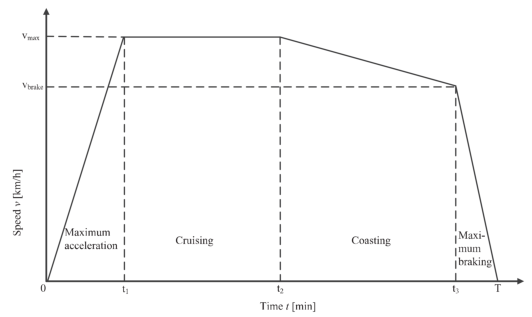
\includegraphics[width=0.5\textwidth,keepaspectratio]{figures/35.DSS/scheepmaker2017a}
		\caption{Optimal traction regimes. Adapted from \cite{scheepmaker2017}.}
		\label{fig:scheepmaker2017a}
	\end{figure}
	
	

\subsection{Timetable scheduling}
\label{subs:353}

	Similarly to Eco-driving \ac{DSS}, in this type of \ac{DSS} is addressed the minimization of the energy consumption, with three research streams in the literature: (1) the usage of the total running time of a train as a variable, (2) the optimal distribution of running time supplements over successive train runs and (3) the synchronization of the timetables to maximize the usage of regenerated braking energy, \cite{scheepmaker2017}.
	
	
	
%\subsection{Maintenance support}
%\label{subs:354}
